\documentclass{senior-design}
\usepackage{lipsum}

%%% Report information %%%%%%%%%%%%%%%%%%%%%%%%%%%%%%%%%%%%%%%%%%
\reporttitle{An Awesome Project Made By An Amazing Student}
% \reporttype{Some types} % Uncomment this line if you want to use \generalreportcover
\semester{Spring 2023}
\sponsor{Prof. \name{Tom}{Jerry}}
\ta{\name{Black}{Shout}}
\reportdate{\today}
\authornames{\nameemail{Kaishen}{Chang}{nehsiak@illinois.edu}}
\addbibresource{references.bib} % The bib database
%%%%%%%%%%%%%%%%%%%%%%%%%%%%%%%%%%%%%%%%%%%%%%%%%%%%%%%%%%%%%%%%%

%%% Project and Team Numbers %%%%%%%%%%%%%%%%%%%%%%%%%%%%%%%%%%%%
\projectnumber{114}
\teamnumber{514}
%%%%%%%%%%%%%%%%%%%%%%%%%%%%%%%%%%%%%%%%%%%%%%%%%%%%%%%%%%%%%%%%%

\begin{document}
\setcounter{page}{1}\pagenumbering{roman}
%%% TITLE PAGE: select the one you need %%%%%%%%%%%%%%%%%%%%%%%%%
\individualreportcover  % coverpage for individual report used for ZJU degree appl.
% \generalreportcover % coverpage for other reports; NEEDS \reporttype{<Type>}
%%%%%%%%%%%%%%%%%%%%%%%%%%%%%%%%%%%%%%%%%%%%%%%%%%%%%%%%%%%%%%%%%
\frontmatter
\thispagestyle{empty}
\newgeometry{left=1in, right=1in, top=1in, bottom=1in}
\begin{center}
    \fontsize{15}{15}\selectfont
    \Large\bfseries Zhejiang University Undergraduate Graduation\\
    Project Report Commitment Statement
\end{center}
\vspace{3em}
{\large\fontsize{11.5}{11.5}\selectfont
\begin{enumerate}
    \item I solemnly promise that the graduation project report submitted was completed in strict accordance with the relevant regulations of the institute and university under the guidance of the project sponsor.
    \item In my graduation project report, except where specifically and explicitly indicated, the report does not contain results that have been published or written by others.
    \item Any contribution to this report made by the teammates with whom I worked has been clearly stated in the report and acknowledged.
    \item I promise that I have not falsified data or committed other similar acts in the completion of the graduation project report.
    \item If there is any infringement of intellectual property rights or breach of academic integrity in this graduation project report, I shall bear the corresponding legal responsibility.
    \item I fully understand that Zhejiang University has the right to retain and send copies and electronic records of this report to relevant departments or institutions. I authorize Zhejiang University to compile all or part of the contents of this report into a relevant database for retrieval and dissemination, and can use photocopying, microprinting or scanning and other means of reproduction to preserve and archive the report.
\end{enumerate}
}
\vfill
\begin{center}
    \fontsize{14}{14}\selectfont
    \hfill
    \begin{minipage}{0.46\linewidth}
        Author's\\
        signature:\\
        ~~~
    \end{minipage}
    \hfill
    \begin{minipage}{0.4\linewidth}
        Project\\
        sponsor's\\
        signature:
    \end{minipage}\\[2em]
    \hfill
    \begin{minipage}{0.46\linewidth}
        Date of\\
        signature:
    \end{minipage}
    \hfill
    \begin{minipage}{0.4\linewidth}
        Date of\\
        signature:
    \end{minipage}
    % \vspace{2em}
\end{center}
\vspace{2cm}
\normalsize
\restoregeometry
\addtocounter{page}{-1}
\clearpage   % commitment statement required by individual report
%%% Abstract %%%%%%%%%%%%%%%%%%%%%%%%%%%%%%%%%%%%%%%%%%%%%%%%%%%%
\chapter*{Abstract}
Put your abstract here

\paragraph{Keywords}
% Put keywords below
Keyword 1, keyword 2, keyword 3

%%% TOC %%%%%%%%%%%%%%%%%%%%%%%%%%%%%%%%%%%%%%%%%%%%%%%%%%%%%%%%%
\tableofcontents
%%%%%%%%%%%%%%%%%%%%%%%%%%%%%%%%%%%%%%%%%%%%%%%%%%%%%%%%%%%%%%%%%

\mainmatter
%%% Body %%%%%%%%%%%%%%%%%%%%%%%%%%%%%%%%%%%%%%%%%%%%%%%%%%%%%%%%
\chapter{Introduction}
\section{Problem statement}
This is a sample document of this template, and here comes citation. You can cite \cite{book1,paper1} and \cite{book2}. However, putting citation at the end of a sentence is also acceptable \cite{webpage1}.
\section{Importance}
\begin{equation}
    f\left( x \right) =\sum_{n=0}^{\infty}{\frac{1}{n!}f^{\left( n \right)}\left( x_0 \right) \left( x-x_0 \right) ^n}, x\in U\left( x_0 \right)
\end{equation}
\begin{equation}
    \begin{aligned}
    e^{ix}&=1+ix+\frac{1}{2!}\left( ix \right) ^2+\frac{1}{3!}\left( ix \right) ^3+\cdots \frac{1}{n!}\left( ix \right) ^n+\cdots
    \\
    &=1+ix-\frac{1}{2!}x^2-i\frac{1}{3!}x^3+\frac{1}{4!}x^4+i\frac{1}{5!}x^5-\cdots
    \\
    &=\left( 1-\frac{1}{2!}x^2+\frac{1}{4!}x^4-\cdots \right) +i\left( x-\frac{1}{3!}x^3+\frac{1}{5!}x^5-\cdots \right)
    \\
    &=\cos x+i\sin x
    \end{aligned}
\end{equation}
\section{Literature Review}
This is a sample listing.
\begin{lstlisting}[language=c]
#include<stdio.h>
void fuzzy(int x){
    return x;
}
int main(){
    int a = 0, b, c;
    scanf("%d", &b);
    c = b;
    if (a == b)
        a = fuzzy(c);
    else
        b = fuzzy(a);
    printf("%d %d\n", a, fuzzy(c));
    return 0;
}
\end{lstlisting}

\chapter{Methodology}

Test the ability\footnote{This is an example footnote.} to print some units, say (in texts), \SI{10e5}{\um\ohm\degree}.

It also applies to equations,
\begin{equation}
    R_{t}=\SI{10e5}{\um\ohm\degree}
\end{equation}

\chapter{Results}
\begin{figure}[H]
    \centering
    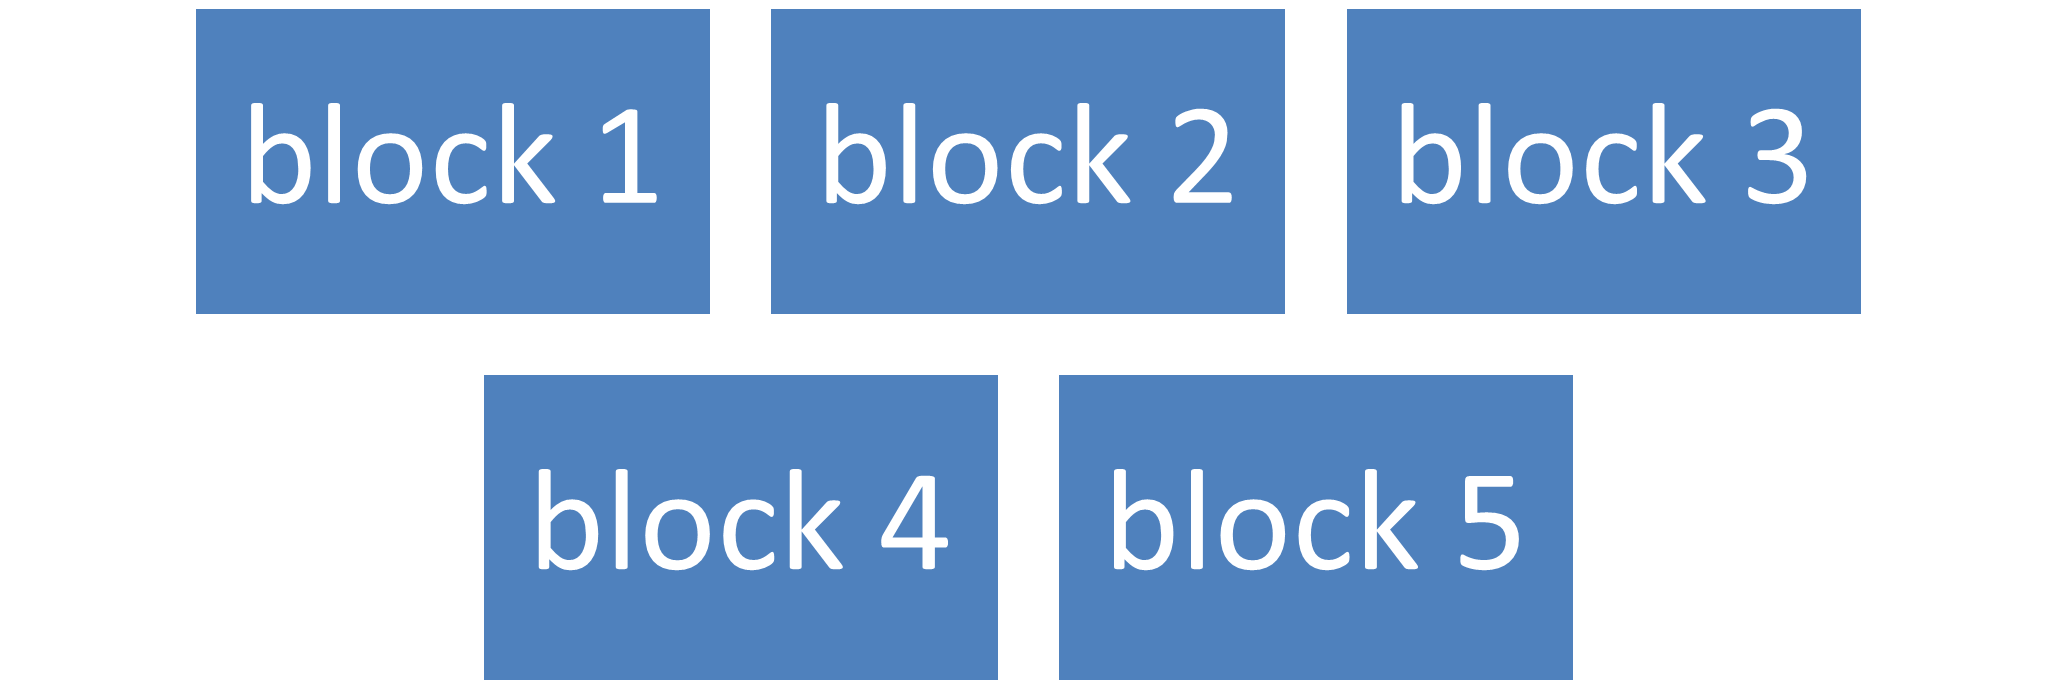
\includegraphics[width=0.8\linewidth]{figs/Picture1.png}
    \caption{An example figure.}
\end{figure}
\chapter{Discussion}

\chapter{Conclusion}

%%%%%%%%%%%%%%%%%%%%%%%%%%%%%%%%%%%%%%%%%%%%%%%%%%%%%%%%%%%%%%%%%

%%% References %%%%%%%%%%%%%%%%%%%%%%%%%%%%%%%%%%%%%%%%%%%%%%%%%%
\clearpage
\renewcommand*{\UrlFont}{\rmfamily}
\printbibliography[title={References},heading=bibintoc]
\clearpage
%%%%%%%%%%%%%%%%%%%%%%%%%%%%%%%%%%%%%%%%%%%%%%%%%%%%%%%%%%%%%%%%%
%%% Appendices %%%%%%%%%%%%%%%%%%%%%%%%%%%%%%%%%%%%%%%%%%%%%%%%%%
\begin{appendices}
% All appendices here, using sections for multiple appendices
\chapter{Example}
An example piece of code:
\lstinputlisting[language=python]{code/example.py}

\section{Some Test Data}

\section{Derivation of Square Law}
\end{appendices}
\clearpage
%%%%%%%%%%%%%%%%%%%%%%%%%%%%%%%%%%%%%%%%%%%%%%%%%%%%%%%%%%%%%%%%%
\backmatter
%%% Acknowledgement %%%%%%%%%%%%%%%%%%%%%%%%%%%%%%%%%%%%%%%%%%%%%
\chapter*{Acknowledgement}
Thank you thank you!
%%%%%%%%%%%%%%%%%%%%%%%%%%%%%%%%%%%%%%%%%%%%%%%%%%%%%%%%%%%%%%%%%
\end{document}